\documentclass{beamer}

\usepackage[utf8]{inputenc} % Ensure proper encoding
\usepackage{graphicx} % For including images
\usepackage{hyperref} % For hyperlinks
\usepackage{amsmath,amsfonts,amssymb} % For mathematical symbols and equations
\begin{document}

\title{Who Is Screened Out? Application Costs and the Targeting of Disability Programs}
\author{Manasi Deshpande \& Yue Li}
\date{\today}

\frame{\titlepage}


\begin{frame}
    \frametitle{Introduction}
    \begin{itemize}
        \item Social Security Disability Insurance (SSDI or DI) provides cash benefits and Medicare to disabled workers in the United States. 
        \item In 2015, it covered nearly 9 million workers.
        \item  Additionally, Supplemental Security Income (SSI) offers cash welfare and Medicaid eligibility to nearly 7 million low-income, disabled Americans, including 1.4 million children in 2015.
        \item This program strictly targets those with severe disabilities who are unable to work.
    \end{itemize}
\end{frame}

\begin{frame}
    \frametitle{This Paper}
    \begin{itemize}
        \item This paper examines the role of application costs in the targeting of disability programs and importantly looks at trade-offs between screening through ordeal and targeting.
        \item The authors use a novel dataset of 1.6 million initial disability applications to estimate the effect of application costs on the composition of program participants using a natural experiment that lead to closing of some field offices that assisted in the application process. 
        \item They find that application costs are a key determinant of program participation, and that the targeting of disability programs is sensitive to the stringency of the application process.
        
    \end{itemize}
\end{frame}

\begin{frame}[allowframebreaks]
    \frametitle{Institutional Background and Data}
    \begin{itemize}
        \item The Social Security Administration (SSA) administers both SSDI and SSI. 
        \item The application process is complex and time-consuming, requiring extensive documentation and medical evidence.
        \item The authors use a novel dataset of 1.6 million initial disability applications to estimate the effect of application costs on the composition of program participants.
        \item The dataset includes all initial disability applications filed between 2006 and 2015, and includes detailed information on the characteristics of applicants, the medical evidence they submit, and the outcomes of their applications.
        \item They use variables such as disability type and severity, age, education, and languages spoken to estimate the effect of application costs on the composition of program participants.
        \item importantly, study channels through which application costs affect the composition of program participants, use office wait times, processing times and staff counts to quantify congestation at neighborhood offices.
    \end{itemize}
\end{frame}
    
\begin{frame}{First Stage}
    \begin{figure}
        \centering
        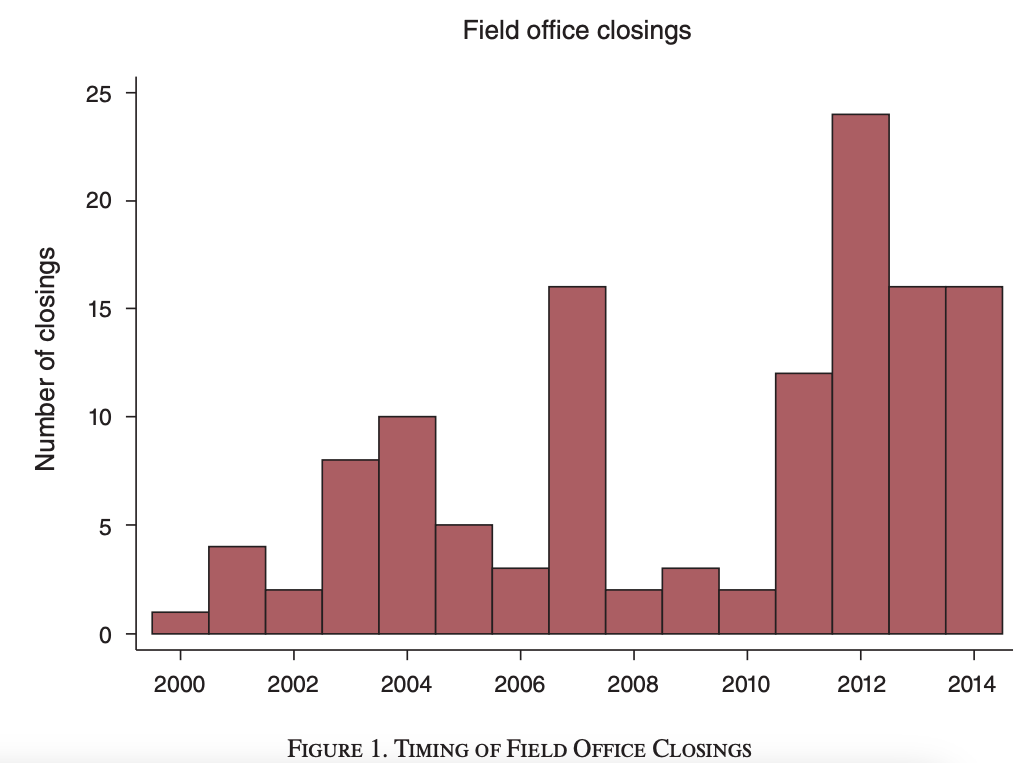
\includegraphics[width=0.8\textwidth]{F1.png}
    \end{figure}
\end{frame}

\begin{frame}{Treated Zip Codes}
    \begin{figure}
        \centering
        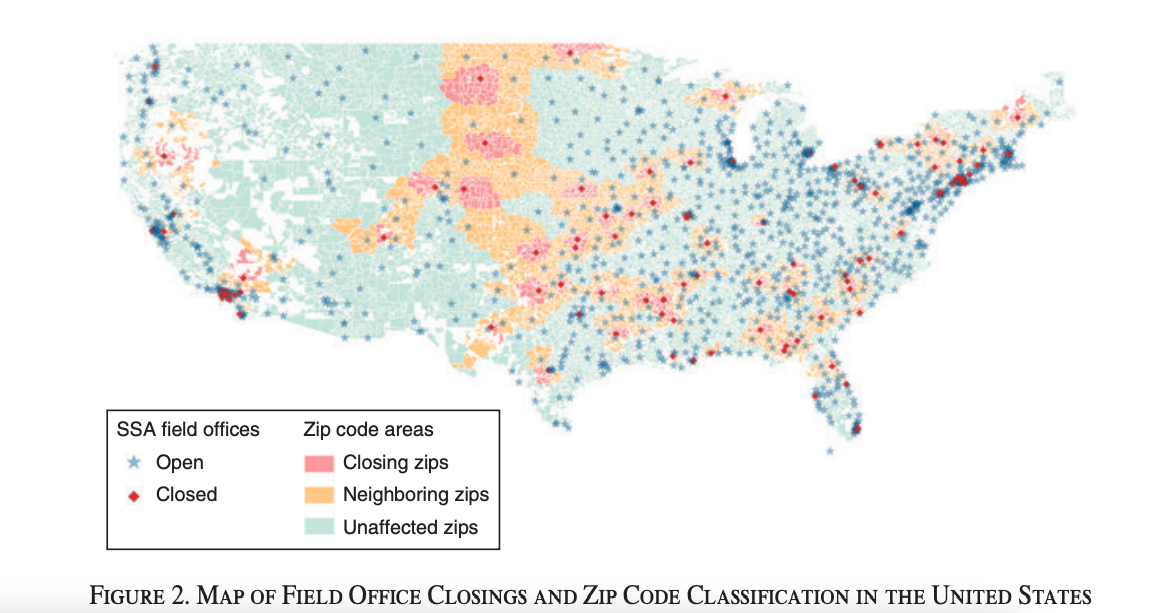
\includegraphics[width=0.8\textwidth]{F2.png}
    \end{figure}
\end{frame}

\begin{frame}{Effect on Applications and Allowances}
    \begin{figure}
        \centering
        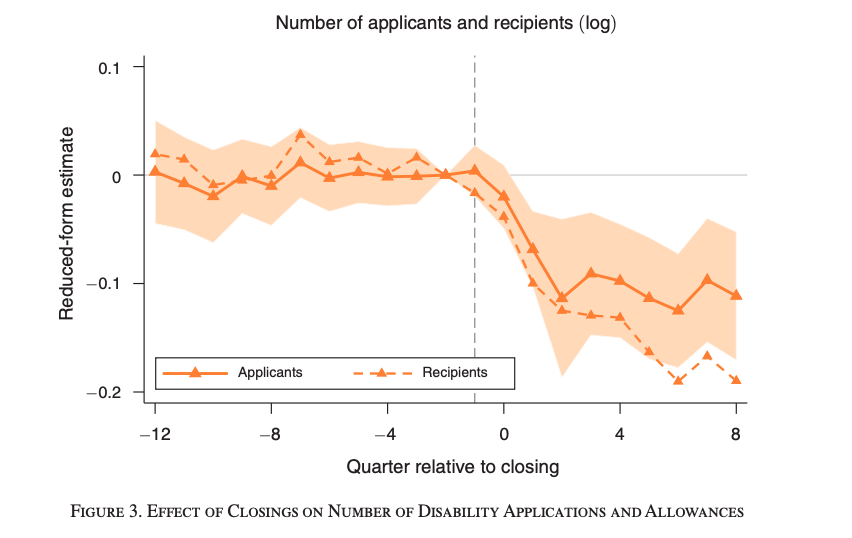
\includegraphics[width=0.8\textwidth]{F3.png}
    \end{figure}
\end{frame}

\begin{frame}{Who is Screened Out?}
    \begin{figure}
        \centering
        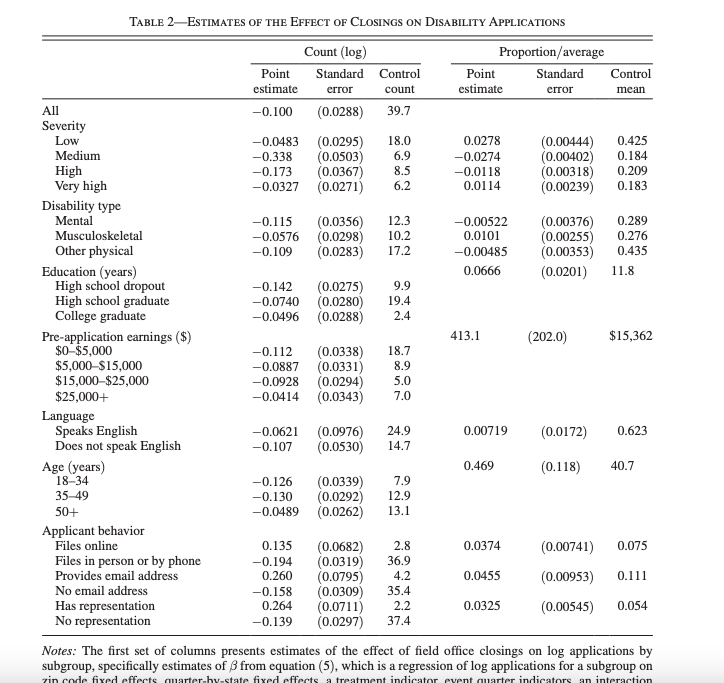
\includegraphics[width=0.8\textwidth]{T2.png}
    \end{figure}
\end{frame}

\begin{frame}{Who is Screened Out?}
    \begin{figure}
        \centering
        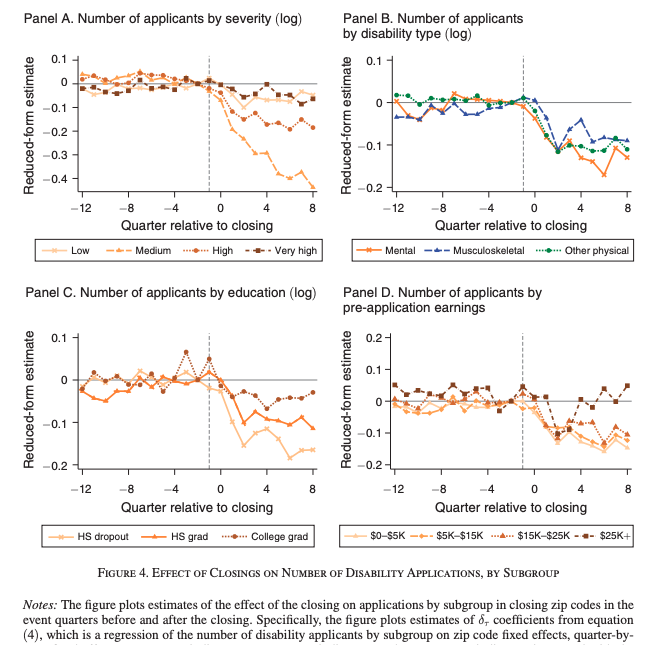
\includegraphics[width=0.8\textwidth]{F4.png}
    \end{figure}
\end{frame}


\begin{frame}{Who is Screened Out?}
    \begin{figure}
        \centering
        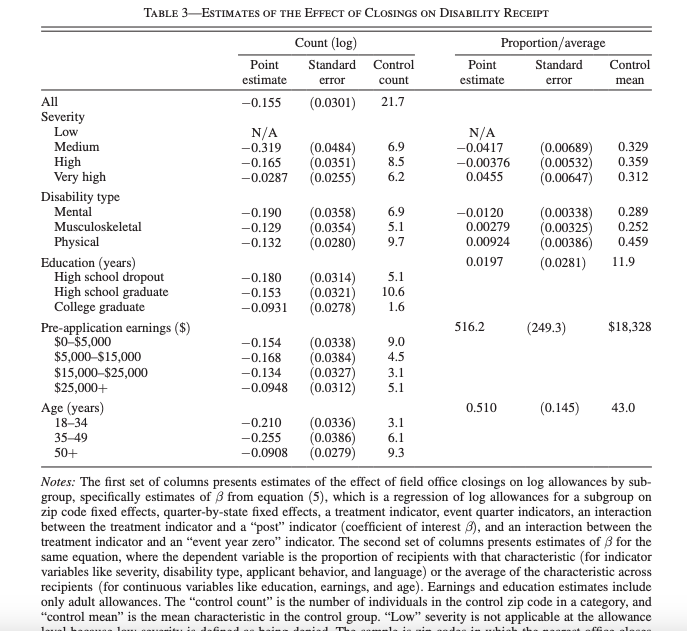
\includegraphics[width=0.8\textwidth]{T3.png}
    \end{figure}
\end{frame}

\begin{frame}{Robustness I}
    \begin{figure}
        \centering
        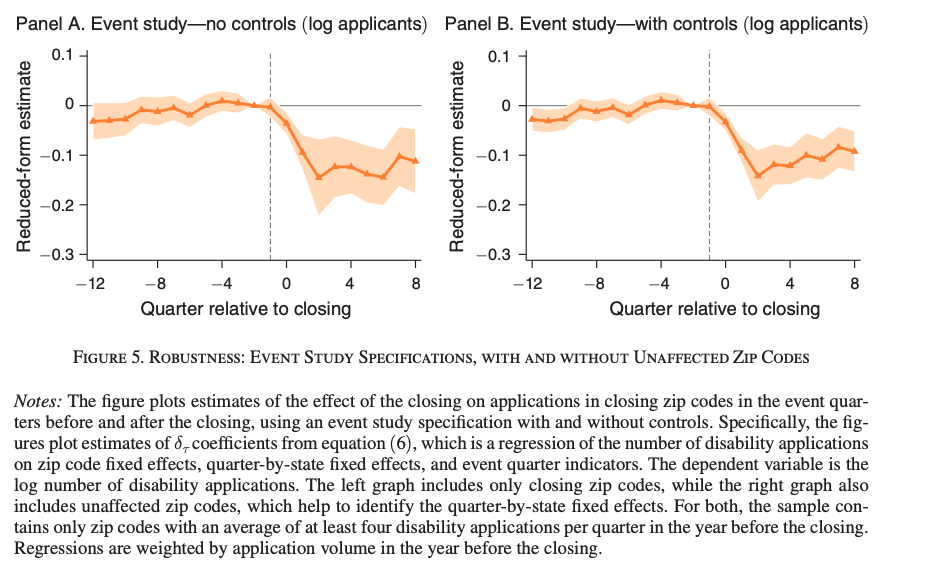
\includegraphics[width=0.8\textwidth]{F5.png}
    \end{figure}
\end{frame}

\begin{frame}{Robustness II}
    \begin{figure}
        \centering
        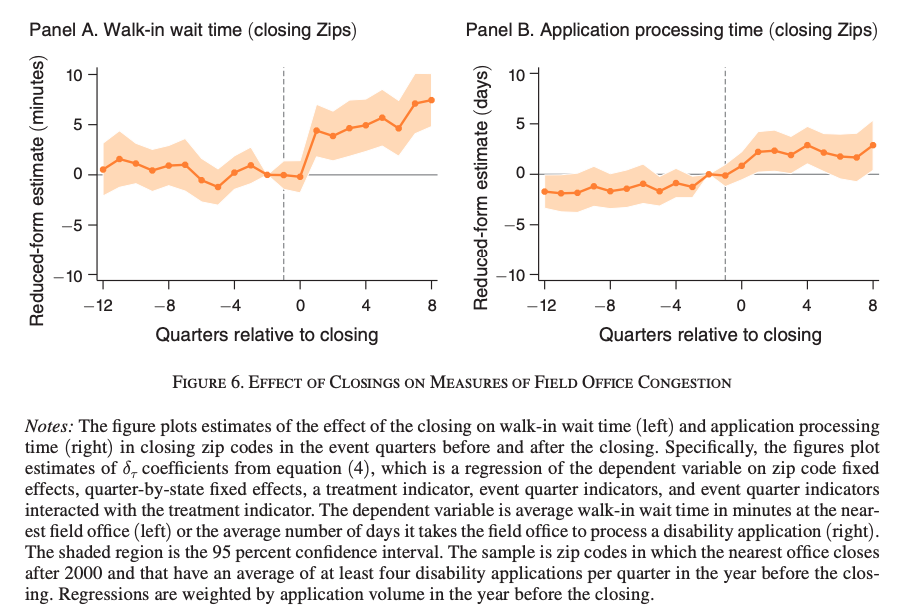
\includegraphics[width=0.8\textwidth]{F6.png}
    \end{figure}
\end{frame}

\begin{frame}{Mechanisms}
    \begin{figure}
        \centering
        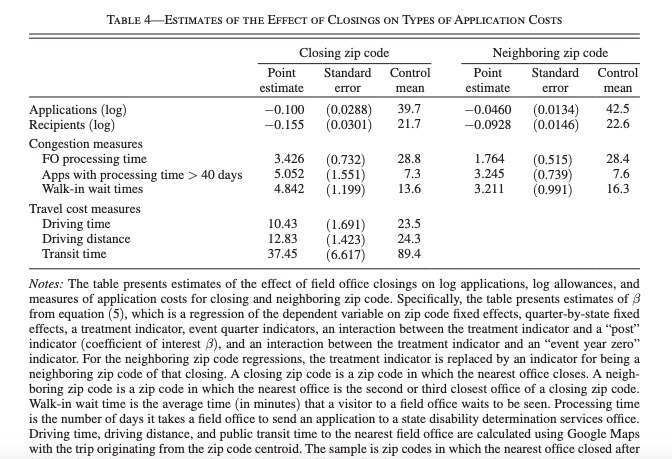
\includegraphics[width=0.8\textwidth]{T4.png}
    \end{figure}
\end{frame}

\begin{frame}{Conclusion}
    \begin{itemize}
        \item The authors find that application costs are a key determinant of program participation, and that the targeting of disability programs is sensitive to the stringency of the application process.
        \item They find that the stringency of the application process affects the composition of program participants, and that the targeting of disability programs is sensitive to the stringency of the application process.
        \item They also find that the stringency of the application process affects the composition of program participants, and that the targeting of disability programs is sensitive to the stringency of the application process.
    \end{itemize}
\end{frame}
    
\end{document}
